\documentclass[10pt]{beamer}

\usepackage[utf8]{inputenc}
\usepackage[T2A]{fontenc}
\usepackage[russian]{babel}
\usepackage{hyperref}
\usepackage{amsmath}
%\usepackage[footnotes,oglav,spisok,boldsect,eqwhole,kursrab,hyperprint]{project1}
\usetheme{Copenhagen}
\useoutertheme{default}
\usecolortheme{sidebartab}
%\usefonttheme{serif}
\useoutertheme[]{miniframes}
\usepackage{graphicx}
\usepackage{lipsum}
%\usepackage{rumathgrk1}
\usepackage{booktabs}
\usepackage{cancel}  % для зачекивания текста
%\usepackage{glonti}
\defbeamertemplate*{footline}{Warsaw} {%
\leavevmode%
\hbox{%
\begin{beamercolorbox}[wd=.5\paperwidth,ht=2.5ex,dp=1.125ex,leftskip=.3cm,rightskip=.3cm]{author in head/foot}%
\insertframenumber{}%
\hfill\insertshortauthor
\end{beamercolorbox}%
\begin{beamercolorbox}[wd=.5\paperwidth,ht=2.5ex,dp=1.125ex,leftskip=.3cm,rightskip=.3cm]{title in head/foot}%
\usebeamerfont{title in head/foot}\insertshorttitle
\end{beamercolorbox}
}%
\vskip0pt%
}
\graphicspath{{images/}}  % папки с картинками

% \setbeamersize
% {
%     text margin left=0.8cm,
%     text margin right=0.8cm
% }
\renewcommand{\thempfootnote}{\arabic{mpfootnote}}
\title{\textbf{Восстановление человеком исходной позы после толчка \\
Reversion of initial posture by a person after a push}}

\author{\textbf{Романов Андрей Владимирович}}
\institute{\textbf{МГУ им. М.В. Ломоносова}\\\textbf{Механико-математический факультет} 
\\ \textbf{Кафедра прикладной механики и управления}
\\ \textbf{Научный руководитель: к.ф.-м.н. Кручинин П.А.}}
\date{\today}



\begin{document}

\maketitle

\begin{frame}{Описание задачи}
	\begin{figure}[h!]
		\begin{center}
			\begin{minipage}[h]{0.33\linewidth}
				\includegraphics[width=0.68\linewidth]{images/human_3.png}
				\caption{Схематическое изображение толкателя
					и положения испытуемого на стабилоплатформе}
			\end{minipage}
			\hfill
			\begin{minipage}[h]{0.66\linewidth}
				\includegraphics[width=1\linewidth]{images/sagg_and_pushes.eps}
				{\footnotesize
					\caption{Координаты центра давления при различных по силе толчках (данные предоставлены сотрудниками ИМБП РАН) }
				}
			\end{minipage}
		\end{center}
	\end{figure}
\end{frame}

\begin{frame}{Задача быстродействия}
	\begin{columns}
		\column{0.55\textwidth}
		\begin{figure}[h!]
			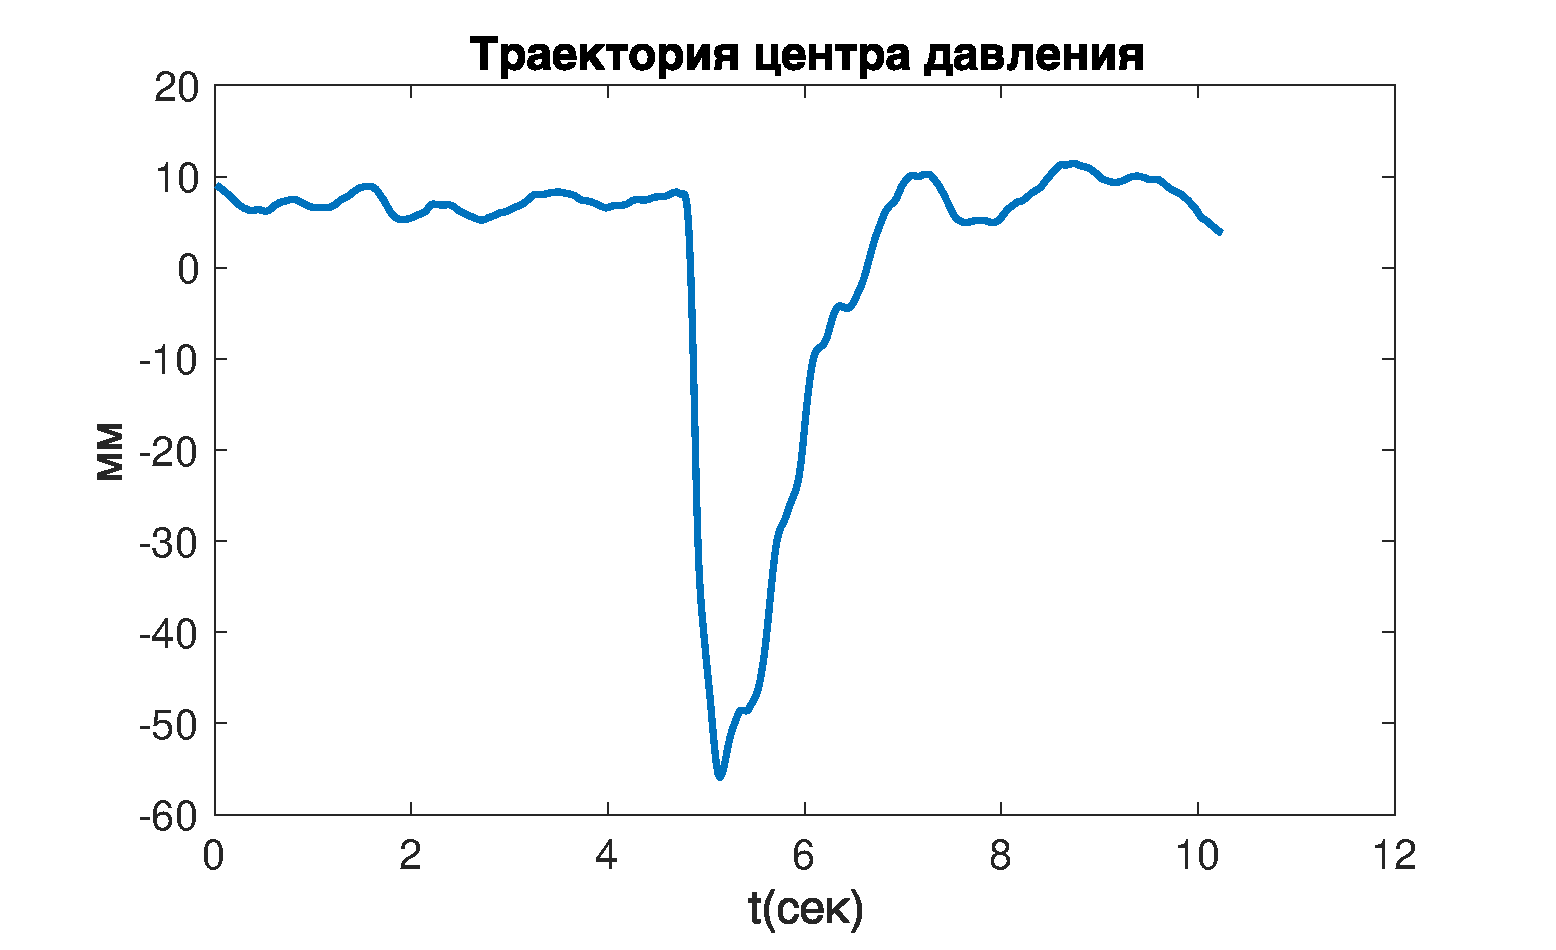
\includegraphics[width=1.1\linewidth]{images/center_of_pressure.eps}
			\caption{Характерный вид сагиттальной стабилограммы при выполнении теста с толчком в грудь}
		\end{figure}
		\column{0.6\textwidth}
		% \column{\dimexpr\paperwidth-2pt}
		В работе рассматриваются возможные алгоритмы управления изменением
		позы человека, основанные на решении задачи оптимального быстродействия,
		которые можно было бы использовать для возвращения человека в исходную
		вертикальную позу. В качестве математической модели используется модель
		«перевернутого маятника». Это решение предлагается использовать для
		оценки эффективности управления человеком при возвращении в
		вертикальную позу, путем сравнения времени реального процесса с полученным
		эталонным решением оптимальной задачи.
	\end{columns}
\end{frame}

\begin{frame}[shrink=8]{Список литературы с опорными исследованиями}
	Разбор аналогичной задачи
	\begin{thebibliography}{15}
		\setbeamertemplate{bibliography item}[book]
		\bibitem{PAKrychinin}П.А. Кручинин Анализ результатов стабилометрических тестов со ступенчатым воздействием с точки зрения механики управляемых систем
		// Биофизика. – 2019. – Т. 64, №5. – С. 1–11.
	\end{thebibliography}

	Исследования в которых был такой же тест
	\begin{thebibliography}{15}
		\setbeamertemplate{bibliography item}[book]
		\bibitem{saenko}Д. Г. Саенко, А. А. Артамонов, И. Б. Козловская Характеристики позных коррекционных ответов
		до и после длительных космических полетов // Физиология человека. – 2011. – Т. 37, №5. – С. 91–99.
		\bibitem{melnikov2}А.А. Мельников, В.В. Филева Методика определения устойчивости вертикальной позы под влиянием
		внешнего толкающего воздействия // Вестник северного (арктического) федерального университета. – 2015. №1. – С. 31–37.
		\bibitem{melnikov}А.А. Мельников, В.В. Филева, М.В. Малахов Эффективность восстановления вертикальной позы
		после толчка у спортсменов разных специализаций // Физиоилогия человека. – 2017. – Т. 43, №4. – С. 78–85.

	\end{thebibliography}

\end{frame}

\begin{frame}{Математическая модель}
	Рассматривается задача возвращения в исходную позу после завершения толчка
	\begin{columns}
		\column{0.62\textwidth}
		\begin{figure}[h!]
			\includegraphics[width=0.55\linewidth]{body_1.pdf}
			\caption{Модель тела человека}
		\end{figure}
		\column{0.5\textwidth}

		\[
			J\ddot{\varphi}=m_Tgl\varphi+M
		\]
		\[
			\varphi(0)=\varphi_0,\, \dot{\varphi}(0)=\omega_0
		\]
		\[
			\varphi(t)=\varphi_k,\, \dot{\varphi}(t_k)=0
		\]
		\[
			M(0)=M(t_k)=-m_Tgl_1\varphi_k
		\]
		\[
			U^-\leqslant\dot{M}\leqslant U^+
		\]
		\[
			\cancel{M^-\leqslant M\leqslant\ M^+.}
		\]



	\end{columns}
\end{frame}
\begin{frame}{Обезразмеривание}
	$\theta - \text{угол отклонения от вертикали}$

	$\omega - \text{угловая скорость тела}$

	$m - \text{момент, возникающий в голеностопном суставе}$


	\begin{columns}
		\column{0.5\textwidth}
		\begin{equation}\label{basesystem}
			\left\{ {\begin{aligned}
						 & \theta^{'} = \omega , \hfill   \\
						 & \omega^{'} = \theta+m , \hfill \\
						 & m^{'} = u . \hfill             \\
					\end{aligned}} \right.
		\end{equation}
		\column{0.5\textwidth}
		\[
			u=
			\begin{cases}
				-u_{max} \\
				+u_{max}
			\end{cases}
		\]\\*
	\end{columns}

	\[
		\tau=\frac{t}{t_\ast},\ t_\ast=\sqrt{\frac{J}{m_Tgl}},\ \varphi_\ast=\varphi_0-\varphi_k
	\]
	\[
		\theta(0)=1;\ \theta^{'}(0)=\frac{t_\ast}{\varphi_\ast}\omega_0=\Omega_0;\ m(0)=0
	\]
	\[
		\theta(\tau_f)=0;\ \theta^{'}(\tau_f)=0;\ m(\tau_f)=0
	\]
\end{frame}
\begin{frame}[shrink=1]{Решение задачи быстродействия}
	Запишем функцию Понтрягина
	\[
		H(\psi(t),y(t),u(t))=\psi_1\cdot\omega+\psi_2\cdot(\theta+m)+\psi_3\cdot u
	\]

	\begin{equation} \label{7}
		\left\{ {\begin{aligned}
					 & \psi^{'}_1=  - \frac{{\partial H}}{{\partial \theta}} = - \psi_2\hfill  \\
					 & \psi^{'}_2=  - \frac{{\partial H}}{{\partial \omega }} = - \psi_1\hfill \\
					 & \psi^{'}_3=  - \frac{{\partial H}}{{\partial m }} = - \psi_2 \hfill     \\
				\end{aligned}} \right.
	\end{equation}
	При $\psi_3\equiv0$ следует, что $\psi_2\equiv0$ и $\psi_1\equiv0$ следовательно особого управления нет.

	Тогда для условия максимизации функции Понтрягина
	\[
		u=
		\begin{cases}
			-u_{max}, & \text{при $\psi_3<0$}          \\
			+u_{max}, & \text{при $\psi_3\geqslant 0$}
		\end{cases}
	\]\\*
	\[
    |u^-|=|\frac{t_\ast U^-}{m_Tgl\varphi_\ast }|=|u^+|=|\frac{t_\ast U^+}{m_Tgl\varphi_\ast}|=|u_\ast|=u_{max}
\]
\end{frame}
\begin{frame}{Решение задачи быстродействия}
	Решая систему \eqref{7}, получим
	\[
		\left\{ {\begin{aligned}
					 & \psi_1 = -C_1e^\tau+C_2e^{-\tau}+C_3, \hfill  \\
					 & \psi_2 = C_1e^\tau+C_2e^{-\tau} , \hfill      \\
					 & \psi_3 = -C_1e^\tau+C_2e^{-\tau}+C_3 . \hfill \\
				\end{aligned}} \right.
	\]
	Анализируя корни уравнения $\psi_3(\tau)=0$, для различной комбинации
	коэффициентов $C_1,C_2,C_3$, получим, что число корней не может быть больше двух. В системе может быть не более двух переключений $u$.

	Пусть первое переключение управления происходит в момент времени
	$\tau=\tau_1$, а второе в момент времени
	$\tau=\tau_2$. Рассмотрим систему \eqref{basesystem} на трех этапах,
	при переходе между которыми меняется управление.


\end{frame}


\begin{frame}{Решение задачи быстродействия}
	Этап 1. $u=-u_*$ начальные условия
	\[
		m(0)=0;\ \theta(0)=1;\ \omega(0)=\Omega_0;
	\]

	\[
		\left\{ {\begin{aligned}
					 & 0 = -\tau  u_*+c_1, \hfill                                                            \\
					 & 1 = \frac{1}{2} e^{-\tau } \left(C_1 \left(e^{\tau }-1\right)^2+C_2 \left(e^{2
					\tau }+1\right)+C_3 e^{2 \tau }-C_3+2 e^{\tau } \tau  u_*\right) , \hfill                \\
					 & \Omega_0 = \frac{1}{2} e^{-\tau } \left(C_1 \left(e^{2 \tau }-1\right)+C_2 \left(e^{2
					\tau }-1\right)+C_3 e^{2 \tau }+C_3+2 e^{\tau } u_*\right)  . \hfill                     \\
				\end{aligned}} \right.
	\]

	\[
		\left\{ {\begin{aligned}
					 & m_1(\tau) = -\tau  u_*, \hfill                                                                         \\
					 & \theta_1(\tau) = \frac{e^\tau+e^{-\tau}}{2}+\frac{\Omega_0-u_*}{2}(e^\tau-e^{-\tau})+\tau u_* , \hfill \\
					 & \omega_1(\tau) =\frac{e^\tau-e^{-\tau}}{2}+\frac{\Omega_0-u_*}{2}(e^\tau+e^{-\tau})+u_*   . \hfill     \\
				\end{aligned}} \right.
	\]
	Аналогично для 2 и 3 этапов
\end{frame}
\begin{frame}{Решение задачи быстродействия}
	Условие сопряжения этих интервалов
	\[
		\left\{ {\begin{aligned}
					 & m_2(\tau_2) = m_3(\tau_2), \hfill            \\
					 & \theta_2(\tau_2) =  \theta_3(\tau_2), \hfill \\
					 & \omega_2(\tau_2) = \omega_3(\tau_2) . \hfill \\
				\end{aligned}} \right.
	\]
	Замена переменных
	\[
		x=e^{\tau_1} ,\,\,y=e^{\tau_2} ,\,\,z=e^{\frac{\tau_f}{2}}
	\]
	\begin{figure}[h!]
		\includegraphics[width=0.8\linewidth]{images/control_intervals.png}
		\caption{Интервалы переключения управления}
	\end{figure}

\end{frame}

\begin{frame}{Решение задачи быстродействия}
	Требуется отобрать наименьший корень уравнений больший 1. При различных по знаку $u_*$.

	\begin{columns}
		\column{1\textwidth}
		\begin{equation}\label{x-y}
			{\begin{aligned}
					 & x=\left( \frac{1}{2z}-\frac{u_*z}{2}-(\Omega_0-u_*)\frac{1}{2z}\right)\frac{z}{u_*(1-z)} \hfill \\
					 & y=zx, \hfill                                                                                    \\
				\end{aligned}}
		\end{equation}
		\begin{equation}\label{koshisystem}
			\left[ {\begin{aligned}
						 & u_*z^2+\Omega _0-1-u_*=0, \hfill                                                            \\
						 & (-u_* \Omega _0+u_*^2-u_*)z^4-4 u_*^2z^3+(2 u_* \Omega _0+6 u_*^2-\Omega _0^2+1)z^2- \hfill \\
						 & -4 u_*^2z+-u_* \Omega _0+u_*^2+u_*=0                                                        \\
					\end{aligned}} \right.
		\end{equation}
	\end{columns}
	$\tau_f=2\ln(z)$

\end{frame}

\begin{frame}{Определение начальных условий для задачи быстродействия}
	Для решения задачи быстродействия необходимо определить начальные условия после толчка.

	\hfill \\
	Для этого необходимо построить оценку $\tilde{\eta}$ траектории центра масс системы, зная траекторию центра давления,
	и взять значение $\tilde{\eta_0}$ и $\tilde{\dot{\eta_0}}$ в момент времени завершения толчка

\end{frame}

\begin{frame}{Связь центра масс и центра давления}
	\begin{columns}
		\column{0.5\textwidth}
		\begin{figure}[h!]
			\includegraphics[width=0.7\linewidth]{body_1.pdf}
			\caption{Силы действующие на модель стержня, имитирующего тело человека}
		\end{figure}
		\column{0.5\textwidth}
		\begin{figure}[h!]
			\includegraphics[width=0.8\linewidth]{images_pres/foot.png}
			\caption{Силы действующие на на систему «стопы ног – платформа стабилоанализатора» }
		\end{figure}
	\end{columns}

\end{frame}

\begin{frame}{Связь центра масс и центра давления}
	\begin{columns}
		\column{0.5\textwidth}
		\begin{equation}\label{init_cond_1}
			\left\{ {\begin{aligned}
						 & ml\ddot{\theta} = -R_y-F , \hfill             \\
						 & 0=R_z-mg, \hfill                              \\
						 & J \ddot{\theta} = mlg\theta-Fl_1+M_x . \hfill \\
					\end{aligned}} \right.
		\end{equation}
		\column{0.5\textwidth}
		\begin{equation}\label{init_cond_2}
			\left\{ {\begin{aligned}
						 & M_x = Ny+F_yh , \hfill \\
						 & F_y = R_y , \hfill     \\
						 & N \approx mg . \hfill  \\
					\end{aligned}} \right.
		\end{equation}
	\end{columns}

	$$M_x=mgy-h\left(F+ml\ddot{\theta}\right)$$

	$$\left(J+mlh\right)\ddot{\theta}=mgl\theta+mgy-Fl_1-Fh$$


	$$\frac{(J+mlh)l\ddot{\theta}}{mgl}=l\theta+y-\frac{F}{mg}(l_1+h);\quad \text{Замена: }\eta=-l\theta; \quad T^2=\frac{J+mlh}{mgl};$$
	\begin{equation}\label{eta_y}
		T^2\ddot{\eta}=\eta-y+\frac{F}{mg}(l_1+h)
	\end{equation}

\end{frame}

\begin{frame}{Связь центра масс и центра давления}
	Cоотношение \eqref{eta_y} используем для определения начальных условий движения сразу после толчка

	\hfill \\
	Далее необходимо построить оценку $\tilde\eta$ движения центра масс различными способами, описанными в работах, выполненых под руководством П.А. Кручинина
\end{frame}


\begin{frame}{Алгоритм фильтрации (композиция двух фильтров)}

	Передаточная функция системы (\ref*{eta_y}) имеет вид
	\[
		G(s)=-\frac{1}{T^2s^2-1}
	\]
	Ее можно представить в виде композиции двух фильтров
	\[
		G(s)=G_1(s)\cdot G_2(s)
	\]
	\[
		G_1(s)=\frac{1}{Ts-1}, G_2(s)=\frac{1}{Ts+1}
	\]
	Оценка координаты центра масс может быть найдена, путем последовательного применения двух фильтров
	\[
		T \dot{x}+x=-y \text{ в прямом времени}
	\]
	\[
		T \dot{\eta}-\eta=x \text{ в обратном времени}
	\]
\end{frame}

% \begin{frame}{Алгоритм фильтрации с использованием преобразования Фурье}
% 	$Y(\omega),N(\omega) - \text{Фурье образы y(t) и $\eta$(t)}$
% 	\[
% 		N(\omega)=G(i\omega)\cdot Y(\omega)
% 	\]
% 	Представим $y(t)=a(t-t_0)+b+\delta(t)$

% 	$a=\frac{y(t_f)-y(t_0)}{t_f-t_0}, b=y(t_0)$, тогда оценка координаты центра масс может быть найдена из

% 	$\eta(t)=a(t-t_0)+b+\chi(t)$, где $\chi(t)$ - Фурье праобраз $N(\omega)$

% \end{frame}


\begin{frame}{Оценка траектории центра масс}
	% \begin{columns}
		% \column{1\textwidth}
		\begin{figure}[h!]
			\centering
			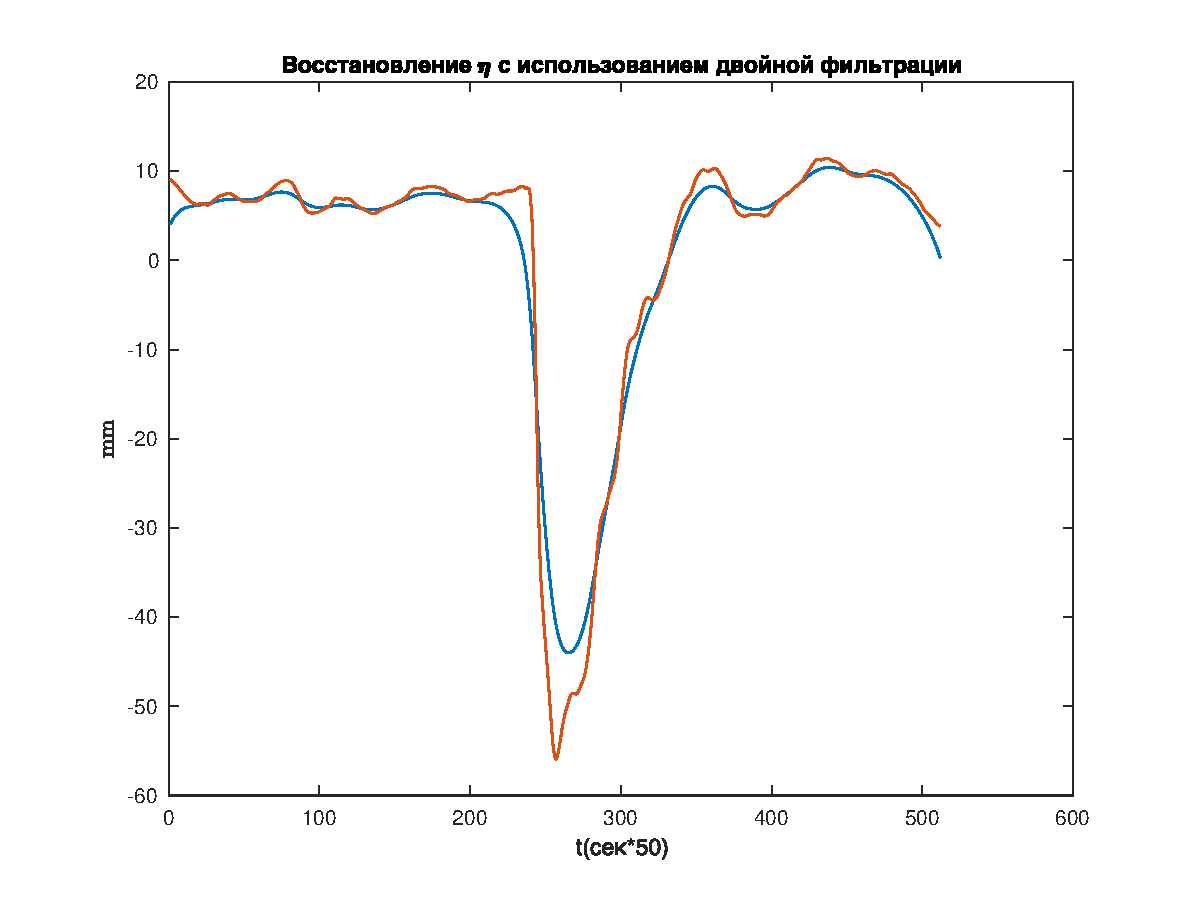
\includegraphics[width=0.8\linewidth]{restore_eta_double_real.eps}
			\caption{Восстановление с использованием двойной фильтрации}
			\label{restore_double_real}
		\end{figure}
	% 	\column{0.5\textwidth}
	% 	\begin{figure}[h!]
	% 		\centering
	% 		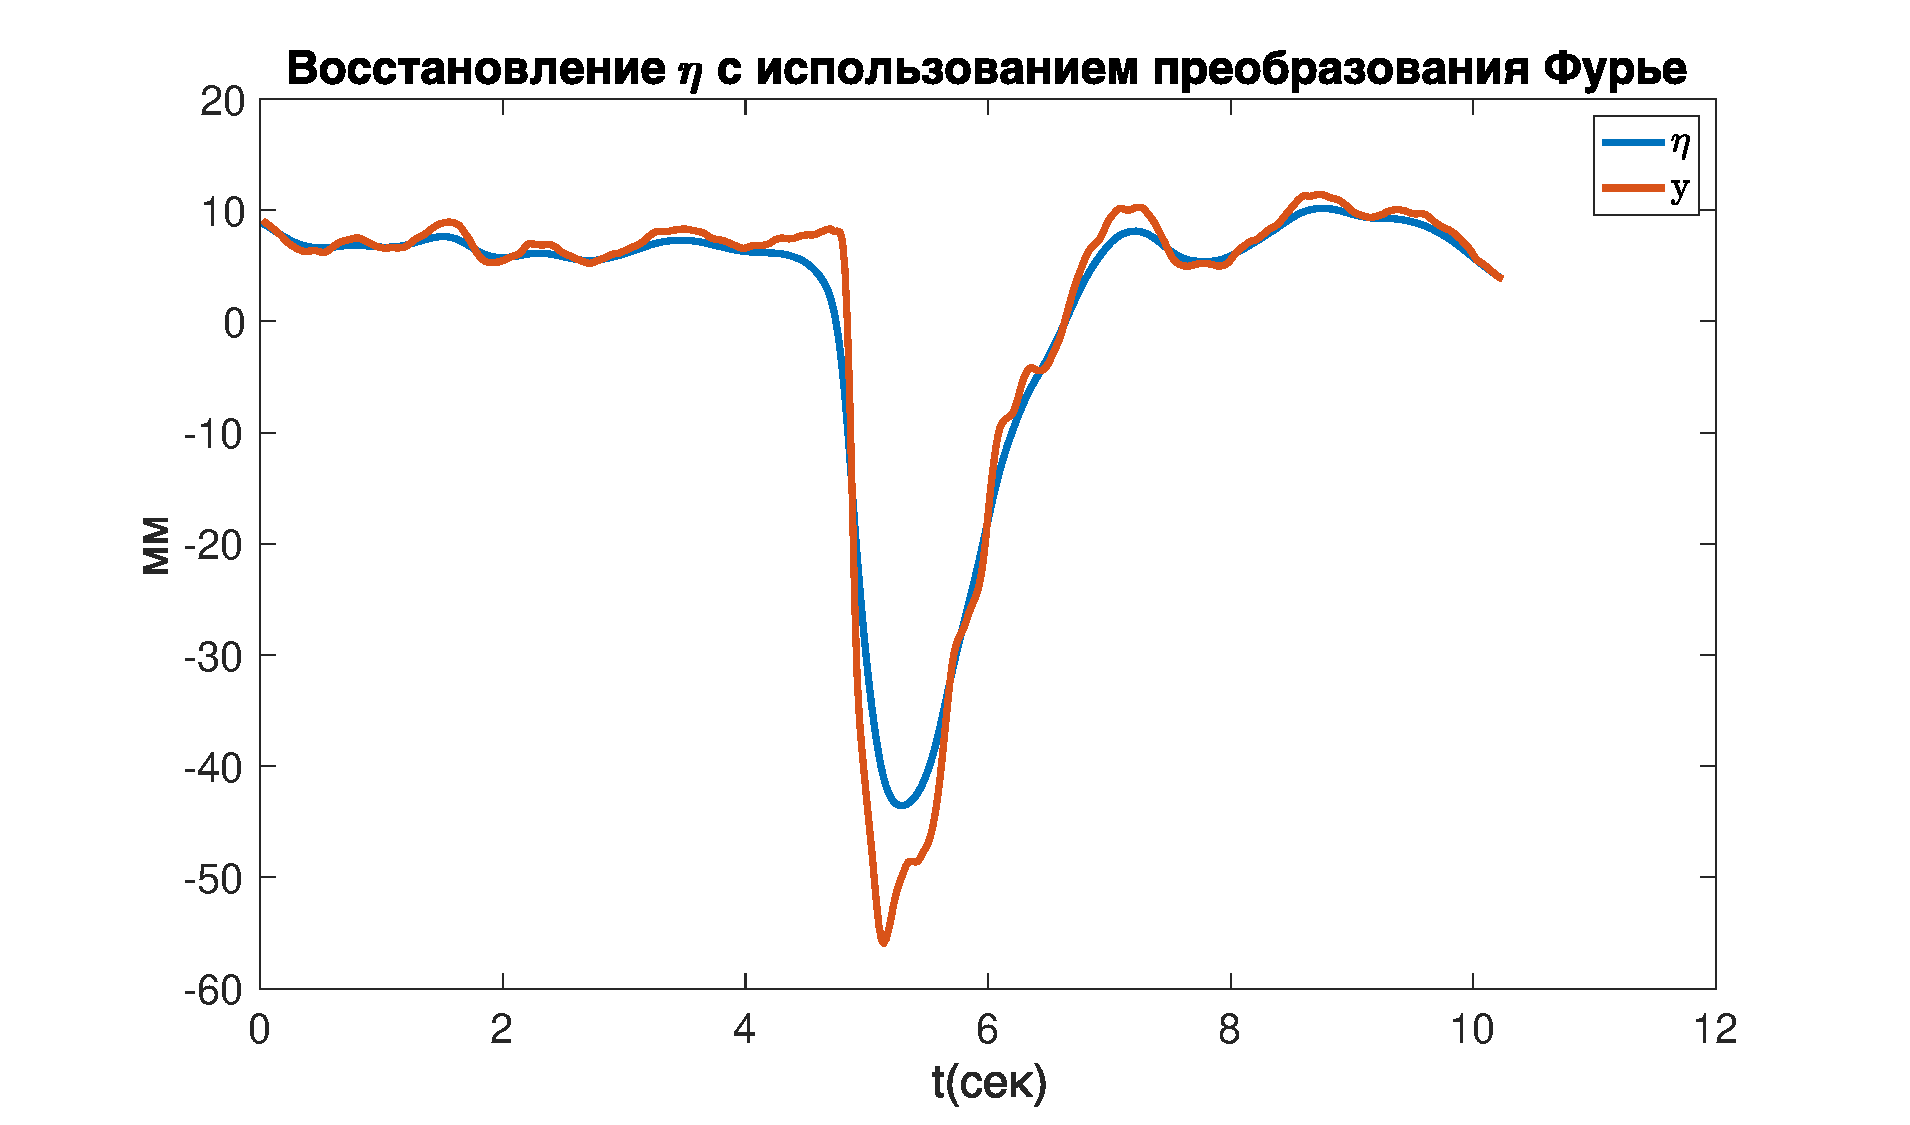
\includegraphics[width=1\linewidth]{restore_eta_fur_real.eps}
	% 		\caption{Восстановление с использованием преобразования Фурье}
	% 		\label{restore_fur_real}
	% 	\end{figure}
	% \end{columns}
\end{frame}
\begin{frame}{Определение начальных условий}
	\begin{figure}[h!]
		\centering
		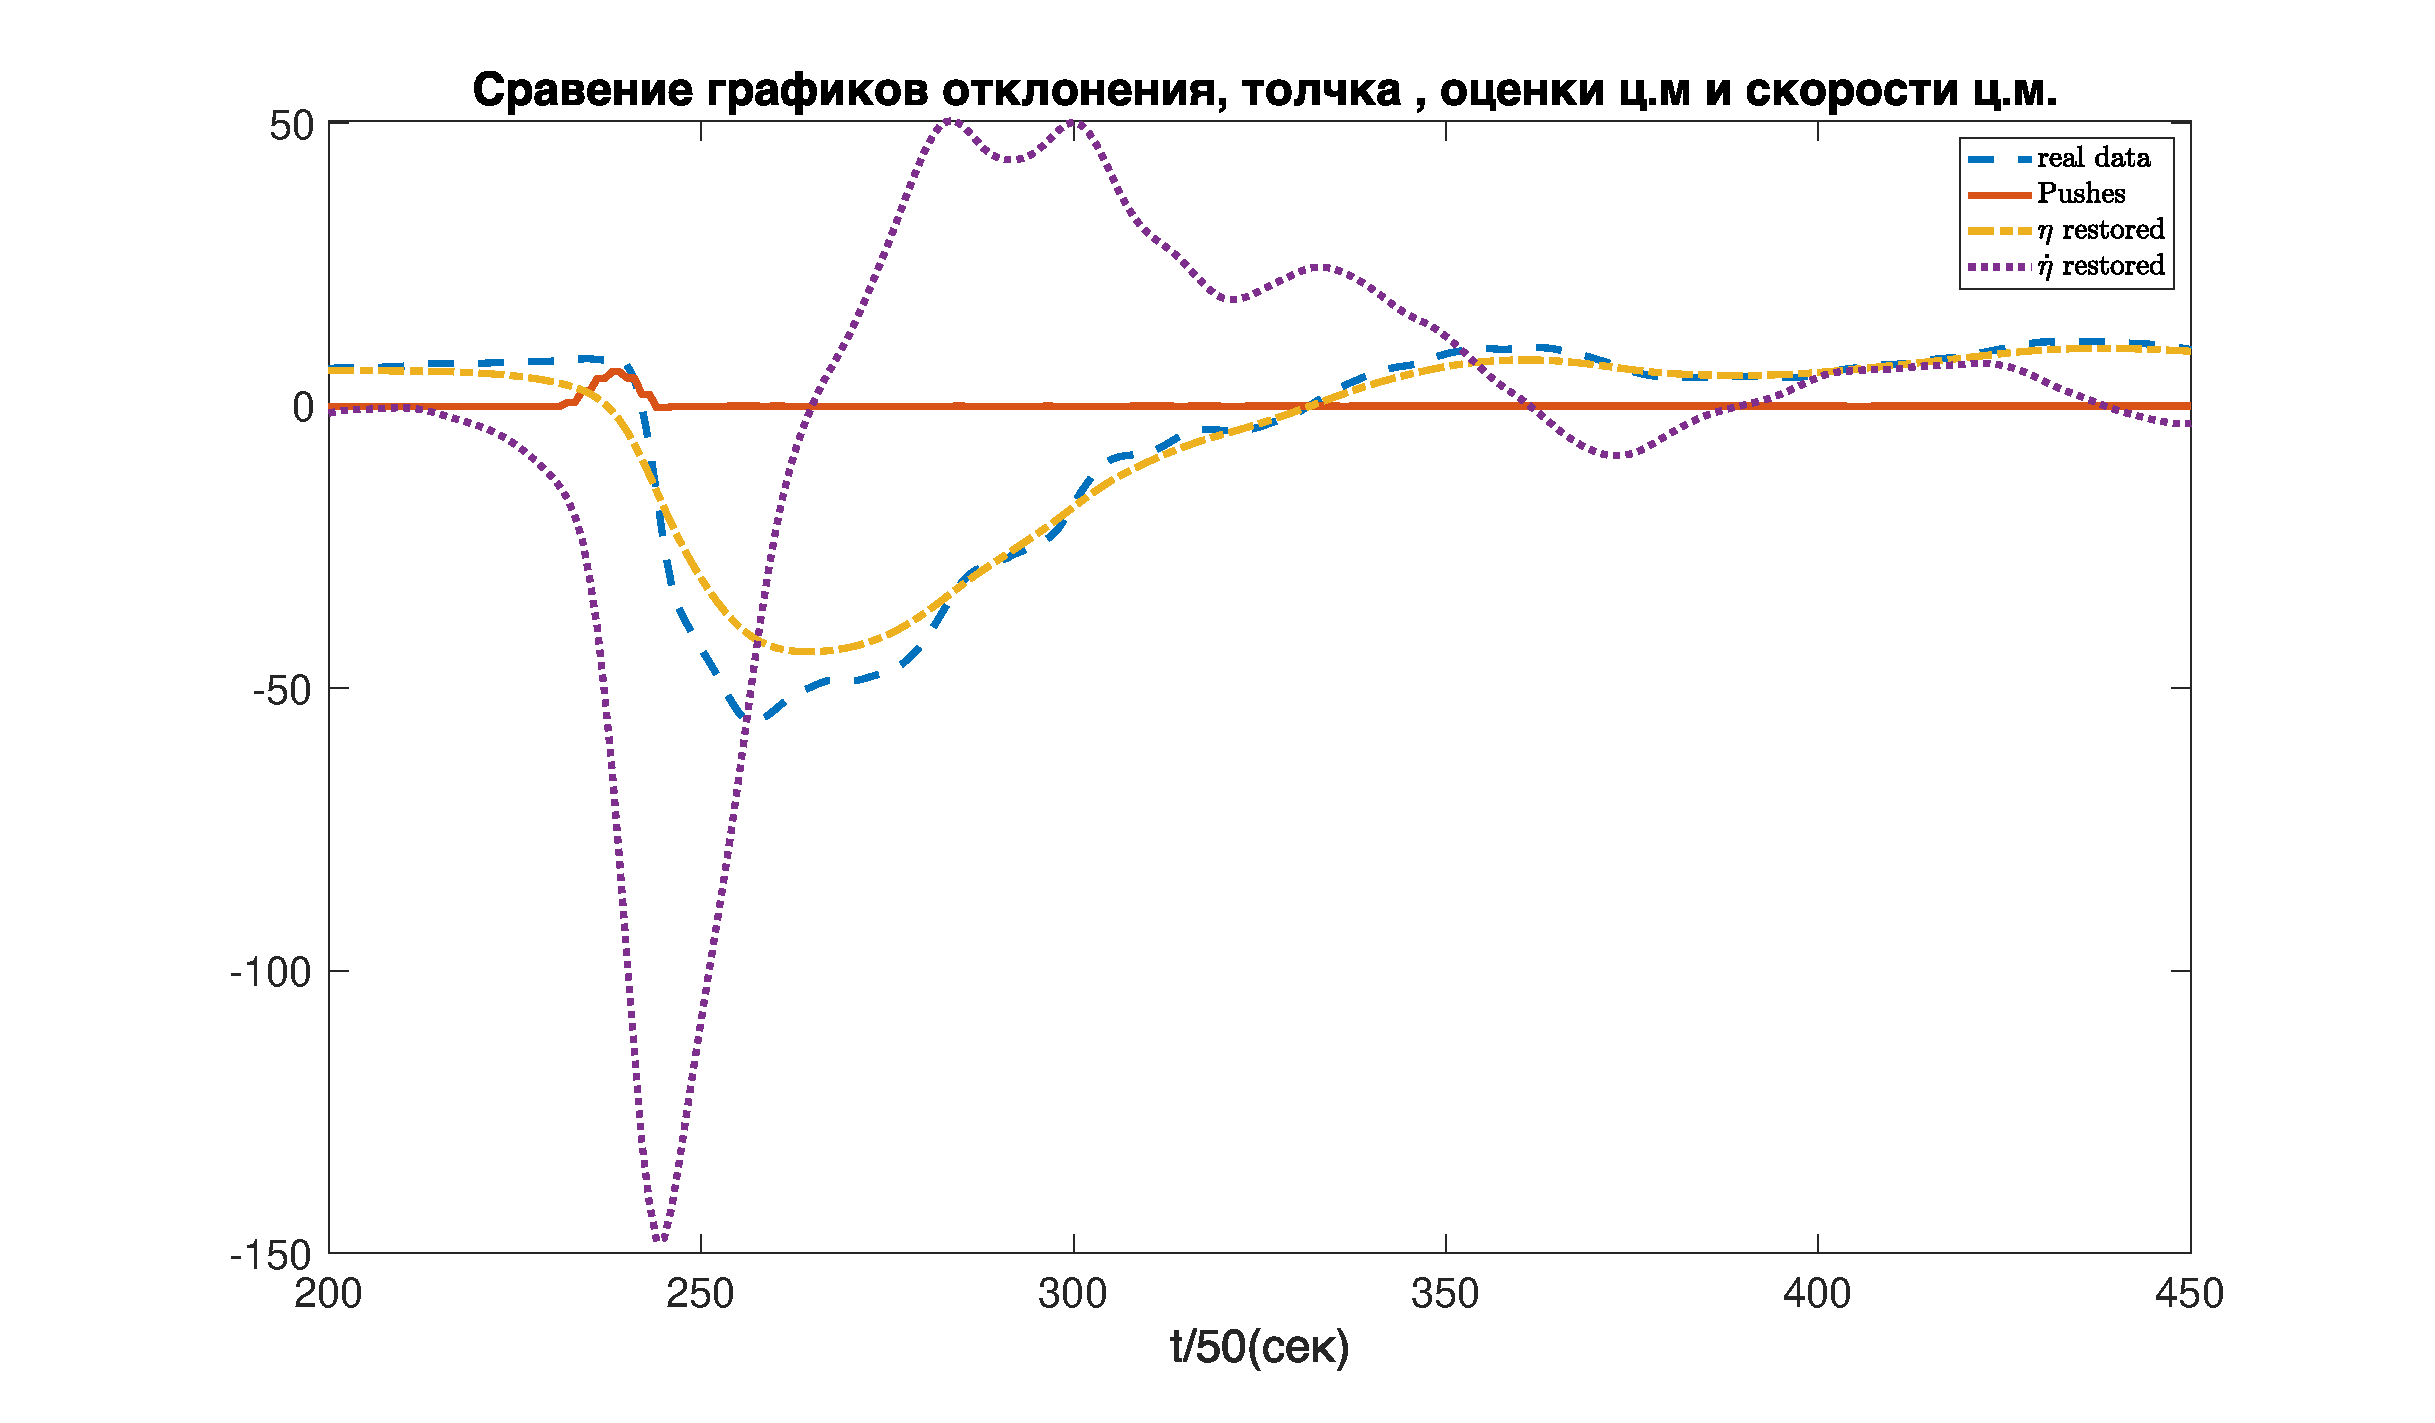
\includegraphics[width=1\linewidth]{images/cp3_bold.eps}
		\caption{К определению начальных условий}
		\label{restore_double_real}
	\end{figure}
\end{frame}

\begin{frame}{Поведение системы при оптимальном управлении}
	При $u_\ast=1.46$, полученном из данных эксперимента, действительных корней уравнения \eqref{koshisystem} больших 1 нет,
	при обоих комбинациях знаков $u_\ast$.
	\begin{figure}[h!]
		\centering
		\includegraphics[width=0.7\linewidth]{3_graphs.jpeg}
		\caption{Оптимальная траектории в безразмерном виде $u_\ast=3.2$ }
		\label{3_graphs}
	\end{figure}
\end{frame}

\begin{frame}{Анализ оптимальных траекторий при различных $u_\ast$}
	\begin{figure}[h!]
		\centering
		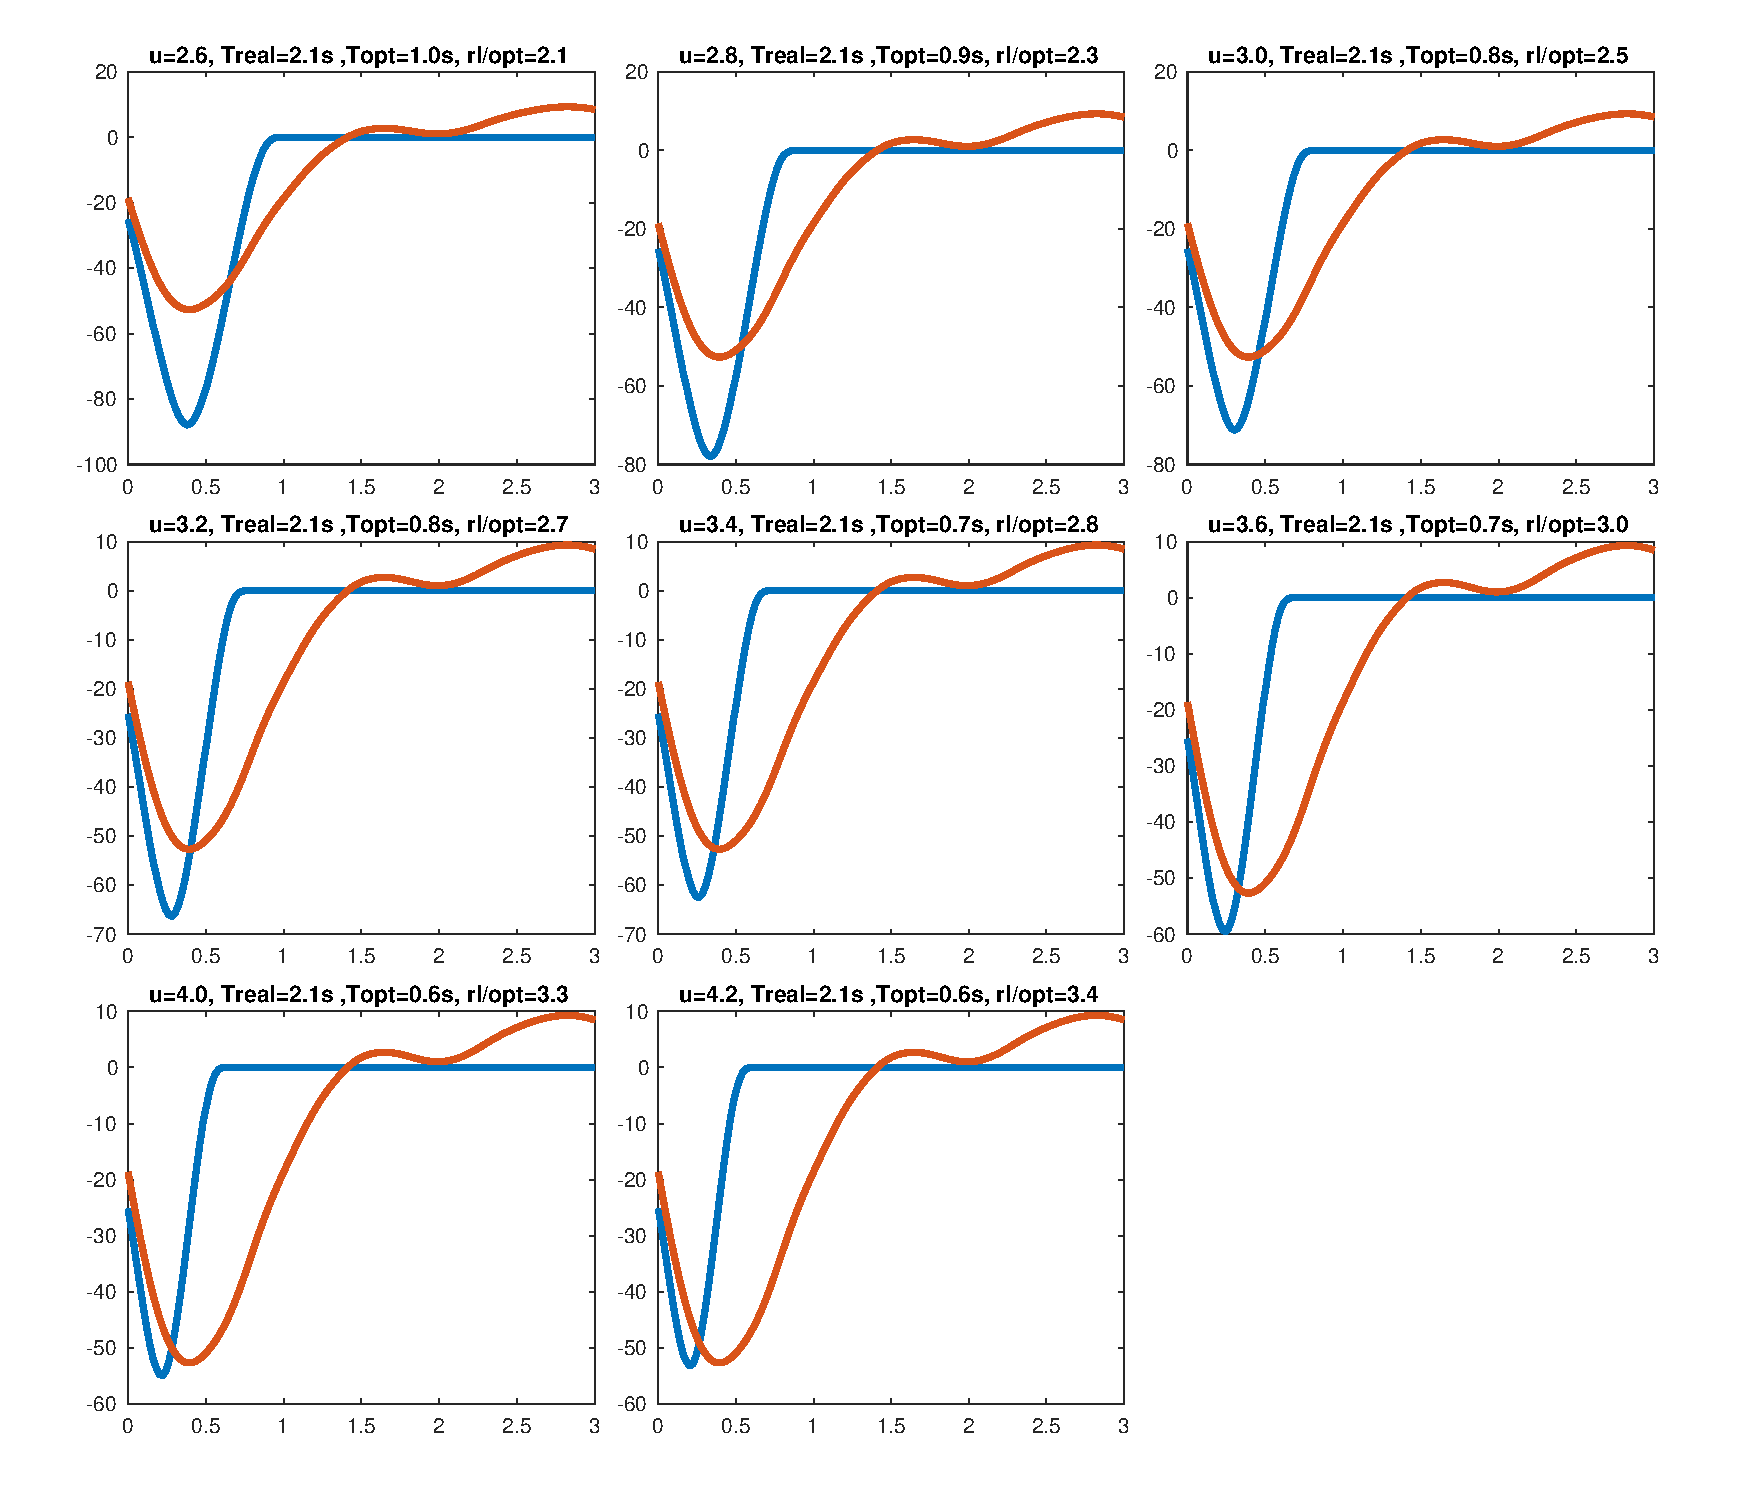
\includegraphics[width=0.9\linewidth]{final_graphs_1.eps}
		\caption{Сравнение характерных оптимальных(пунктирные) и реальных(сплошные) траектории на возвратном движении человека}
		\label{final_graphs_1}
	\end{figure}
\end{frame}
\begin{frame}[shrink=21]{Анализ траекторий на выборке толчков}
	Для различных толчков, с примерно одинаковой силой отношение $\dfrac{T_{real}}{T_{opt}}$ остается постоянным.
	\begin{table}[h!]
		\centering
		\begin{tabular}{|l|c|c|c|c|c|c|c|c|c|}
			\hline
			\textbf{Номер толчка}       & \textbf{1} & \textbf{2} & \textbf{3} & \textbf{4} & \textbf{5} & \textbf{6} & \textbf{7} & \textbf{8} & \textbf{9} \\ \hline
			\textbf{$F_{max}$(Н)}       & 6.01       & 6.87       & 8.21       & 8.56       & 9.73       & 4.74       & 5.49       & 1.97       & 3.3        \\ \hline
			\textbf{Время толчка(сек)}  & 0.26       & 0.26       & 0.26       & 0.26       & 0.26       & 0.26       & 0.26       & 0.26       & 0.26       \\ \hline
			\textbf{$\varphi_0$ рад}    & 0.026      & 0.028      & 0.033      & 0.033      & 0.035      & 0.022      & 0.018      & 0.008      & 0.007      \\ \hline
			\textbf{$\omega_0$ рад/с}   & 0.15       & 0.18       & 0.17       & 0.20       & 0.21       & 0.10       & 0.15       & 0.05       & 0.08       \\ \hline
			\textbf{Момент(Н$\cdot$м)}  & 14.88      & 19.21      & 17.95      & 19.28      & 19.95      & 9.97       & 14.16      & 6.38       & 7.95       \\ \hline
			\textbf{real/opt $u_*=3.2$} & 2.8        & 2.7        & 2.8        & 2.8        & 2.9        & 2.7        & 1.8        & 1.8        & 2.0        \\ \hline
			\textbf{real/opt $u_*=3.6$} & 3.1        & 3.0        & 3.1        & 3.1        & 3.2        & 2.9        & 2.0        & 2.0        & 2.3        \\ \hline
		\end{tabular}
		\caption{Анализ различных толчков}
		\label{final_table}
	\end{table}
\end{frame}
\begin{frame}
	В ходе работы:
	\begin{itemize}
		\item Показано, что решение оптимальной задачи быстродействия при ограниченной
		      скорости изменения момента в голеностопном суставе может иметь решение, которое качественно совпадает с картиной, наблюдаемой в стабилометрических исследованиях;
		\item Представлено аналитическое решение задачи быстродействия;
		\item Найдены начальные условия в момент завершения толчка, с помощью метода двойной фильтрации;
		\item Время необходимое для восстановления исходной позы получилось
		      соизмеримым с реальным времени возвращения после толчка;
		\item Проведен анализ допущений, которые могут скорректировать соответствие математической модели и реального процесса.
	\end{itemize}
\end{frame}
\begin{frame}
	\centering{{\huge Спасибо за внимание!}}
\end{frame}
\end{document}